\documentclass[../main.tex]{subfiles}

\begin{document}

\section{System Architecture}\label{sec:systemarchitecture}

The system architecture of PlaceAdvisor is designed to be a robust and scalable solution for providing information on points of interest and facilitating user interactions. The architecture is based on microservices, with each component responsible for specific tasks and functionalities. Below is an overview of the key architectural components and technologies used:

\begin{figure}[H]
	\centering
	\label{fig:pngegg}
	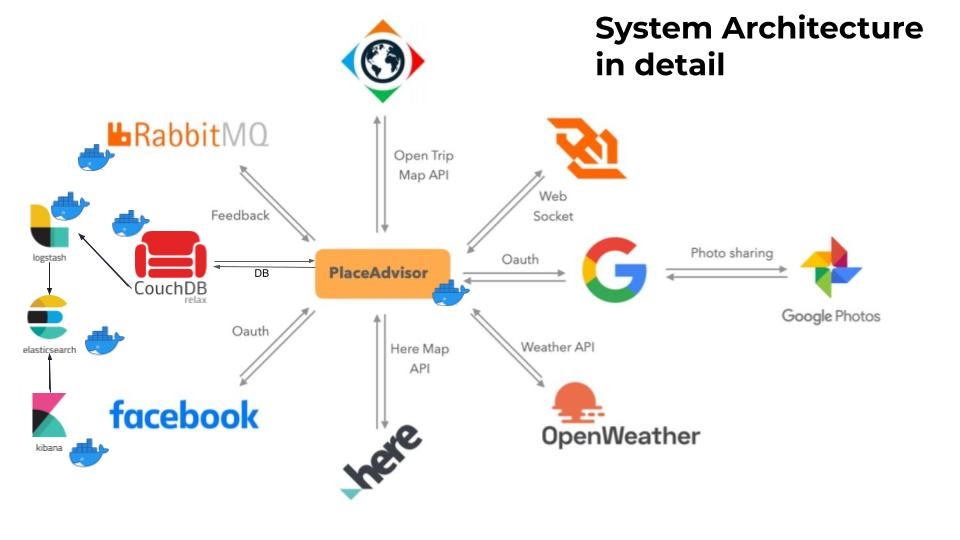
\includegraphics[width=1\linewidth]{../figures/System Architecture.jpg}
  \end{figure}

\subsection{Microservices}

PlaceAdvisor employs a microservices architecture, which allows for modularity and flexibility in scaling individual components. The following microservices make up the system:

\begin{enumerate}
    \item \textbf{Node.js Service:} This microservice is responsible for handling user registration, authentication, and user-related operations. It communicates with the CouchDB database to store user data and interacts with external services for authentication.
    
    \item \textbf{CouchDB:} A NoSQL database used for storing user information, city data, and user reviews. It provides a scalable and reliable data storage solution for the application.
    
    \item \textbf{RabbitMQ:} A message broker used for handling asynchronous tasks and feedback processing. It ensures reliable communication between components and allows for scaling services independently.
    
    \item \textbf{Elasticsearch and Kibana:} Elasticsearch serves as the search and analytics engine for user reviews and places of interest. Kibana provides a user-friendly interface for data visualization and exploration.
    
    \item \textbf{Logstash:} Logstash is responsible for collecting and processing data from couchdb and to use them in elasticsearch.
    
    \item \textbf{Support Service:} This microservice handles user feedback and support-related operations.
\end{enumerate}

\subsection{Integration with External Services}

PlaceAdvisor integrates with several external services to enhance its functionality and user experience. These services include:

\begin{enumerate}
    \item \textbf{OpenTripMap API:} Used to obtain information about places of interest, including their details, locations, and categories.
    
    \item \textbf{OpenWeatherMap API:} Provides real-time weather data for locations, enhancing the user's experience with weather information.
    
    \item \textbf{HERE API:} Enables the identification of places on a map, allowing users to visualize the location of points of interest.
    
    \item \textbf{Google Photos and OAuth:} Users can upload photos in their reviews. OAuth is used for secure and authorized access to Google Photos.
    
    \item \textbf{Facebook OAuth:} Allows users to log in to PlaceAdvisor using their Facebook credentials and share posts if desired.
\end{enumerate}

\subsection{Messaging and Communication}

To ensure efficient communication and data exchange between components for the feedback service, PlaceAdvisor relies on the RabbitMQ message broker. This allows for asynchronous processing of tasks such as feedback handling, ensuring system responsiveness and scalability.


\subsection{Data Storage and Persistence}

CouchDB is used as the primary database for storing user data, city information, and user reviews. It provides the required flexibility and scalability for a system that handles user-generated content.

\subsection{Web Socket}

Web Sockets are used to implement a chat between the user and the support. The communication happens in real-time and it is realized with the purpose of offering a service to the user which can increase the user-friendlyness of the website.

\subsection{Security}

The system ensures secure communication using OpenSSL for HTTPS connections, protecting user data and interactions.

\end{document}